\documentclass[11pt,a4paper]{article}

\usepackage[T1]{fontenc}
\usepackage[utf8]{inputenc}
\usepackage{lmodern}
\usepackage{microtype}
\usepackage[margin=25mm]{geometry}
\usepackage{amsmath,amssymb,amsthm,mathtools}
\usepackage{booktabs}
\usepackage{array}
\usepackage{longtable}
\usepackage{seqsplit}
\let\unbrokentexttt\texttt
\renewcommand{\texttt}[1]{\unbrokentexttt{\seqsplit{#1}}}
\usepackage{enumitem}
\usepackage{tikz}
\usepackage[hidelinks]{hyperref}
\usepackage{url}
\urlstyle{tt}
\usetikzlibrary{arrows.meta,positioning,shapes.misc}

\newtheorem{theorem}{Theorem}[section]
\newtheorem{proposition}[theorem]{Proposition}
\newtheorem{lemma}[theorem]{Lemma}
\newtheorem{corollary}[theorem]{Corollary}
\newtheorem{conjecture}[theorem]{Conjecture}
\theoremstyle{definition}
\newtheorem{definition}[theorem]{Definition}
\newtheorem{question}[theorem]{Research Question}

\newcommand{\Tval}{\mathbf{T}}
\newcommand{\Fval}{\mathbf{F}}
\newcommand{\Bval}{\mathbf{B}}
\newcommand{\Nval}{\mathbf{N}}
\newcommand{\Bel}{\mathsf{B}}
\newcommand{\Know}{\mathsf{K}}
\newcommand{\Stable}{\mathsf{Stable}}
\newcommand{\Ppos}{P^{+}}
\newcommand{\Pneg}{P^{-}}
\newcommand{\thr}{c}
\newcommand{\dthr}{d_{\mathrm{thr}}}
\newcommand{\side}{\operatorname{side}}
\newcommand{\cond}{\mid}
\newcommand{\llbracket}{\mathopen{[\![}}
\newcommand{\rrbracket}{\mathclose{]\!]}}
\newcommand{\statusverified}{\textup{\textsc{Status: Proved; trust inventory in Appendix~\ref{app:formal}.}}}
\newcommand{\statuswitness}{\textup{\textsc{Status: Finite-witness; trust inventory in Appendix~\ref{app:formal}.}}}
\newcommand{\statusinterpretive}{\textsc{Status: structural interpretation.}}
\newcommand{\statusopen}{\textsc{Status: open.}}

\title{From Threshold Belief to Epistemic Phase Geometry:\\Mechanized Dynamics in a Four-Valued Probabilistic Epistemic Logic}
\author{Julian L. Voigt (cr4bbz)}
\date{Working manuscript, version 0.7, 8 September 2026}

\begin{document}
\maketitle

\begin{abstract}
I investigate how four-valued evidence changes under probability-only conditionalization and what is lost when quantitative support is reduced to categorical belief. In the 4-PEL semantics, belief thresholds positive and negative support separately. A primitive, qualitative operator called evidence-stable knowledge returns that belief value on homogeneous accessible profiles and strict falsity otherwise. The term ``knowledge'' denotes this stipulated operator, not an independently established theory of epistemic justification.

A six-world witness family realizes all sixteen source--target values of \(\Know(\Bel p)\). For a chosen rational affine interpolation of support endpoints, threshold-bit changes determine unique wall-hit parameters; their order determines adjacent intermediate states. These parameters describe the interpolation, not an inferred history of the discrete update. Separately, normalized nonnegative world weights yield certified finite measures and convex model-valued paths whose fixed-event masses are affine. Formula-level identification for probability-sensitive events and generation of intermediate models by conditionalization remain open.

A further six-cell refinement records reliability tags while preserving four-cell support and convex mixing. Fine modal stability is equivalent to coarse stability plus local fibre rigidity; explicit S5-frame counterexamples show that coarse stability alone loses reliability information. This is a semantic projection result, not an axiomatization of a six-valued logic.

At the coarsest evidence level, the bilateral positive/negative signature induces a two-class matroid closure: same-polarity atoms are parallel, closure preserves the four-valued state, and the channel ranks of \(\Nval,\Tval,\Fval,\Bval\) are respectively \(0,1,1,2\). The interaction with the existing topological evidence semantics has an exact boundary: topological closure satisfies the repository's exchange axiom exactly when singleton specialization is symmetric, the \(R_0\) condition for genuine topological spaces. The existing Sierpiński witness fails this boundary, while the coarse positive/negative channel matroid is recovered as the closure of its canonical partition topology.

The circuit structure of this coarse matroid is completely classified: minimal dependent evidence sets are exactly distinct same-polarity pairs. Such a circuit generates the same coarse closure as either retained member, making ``minimal redundancy'' precise at the projected level. A contraction-style background construction further shows that accepting one atom makes all same-polarity parallel atoms loop-like over empty new evidence, while the opposite channel remains ungenerated. These are structural theorems about the 4-PEL projection, not claims that arbitrary epistemic evidence is matroidal.

The Lean 4.31 artifact distinguishes the lightweight model interface from probability-integrity-certified models and records declaration-level axiom dependencies, rejecting native evaluation in the selected manuscript proof chains. The contribution is a mechanized case study with explicit preservation and information-loss boundaries; no completeness, general continuity, or priority claim is made.
\end{abstract}

\section{Introduction}
\label{sec:introduction}

Probabilistic epistemic models are usually asked two different questions. One concerns degrees: how much support does an agent assign to a proposition? The other concerns categories: does the agent believe, know, reject, or remain undecided? Threshold approaches connect the two by turning sufficiently high probability into all-or-nothing belief. Four-valued semantics adds a second axis. Positive and negative support can coexist or both fail, so the categorical result is no longer binary but belongs to
\[
  \{\Tval,\Fval,\Bval,\Nval\}
  =\{(1,0),(0,1),(1,1),(0,0)\},
\]
following the Belnap--Dunn/FDE tradition \cite{Belnap1977,Dunn1976}.

The 4-PEL project combines these ideas in a finite-accessibility evidence semantics. Positive and negative extensions are measured separately by the same local set function. A Lockean threshold is applied to each mass, producing a four-valued belief state. A separate evidence-stable knowledge operator then checks whether the complete FDE profile is invariant across the accessible range. This yields an exact factorization:
\[
  \Know_i\varphi=
  \begin{cases}
    \Bel_i\varphi,&\Stable_i(\varphi),\\
    \Fval,&\text{otherwise.}
  \end{cases}
\]
The knowledge operator is therefore not a second probability threshold. It is a qualitative stability filter on top of threshold belief.

The lightweight interface and its stronger probability-certified subclass are distinguished in Section~\ref{sec:kernel}. The paper studies one-step conditionalization and, separately, a chosen affine interpolation of its support endpoints:

\begin{question}[Dynamic phase geometry]
Which four-valued belief and knowledge endpoints can admissible conditionalization connect, and what additional phase structure follows if their signed supports are interpolated affinely?
\end{question}

The machine-checked answer develops in several layers. First, admissible conditionalization can both destroy and restore the stability gate. More strongly, a fixed six-world construction scheme realizes every ordered pair of four-valued values at the level of \(\Know(\Bel p)\). Thus the categorical reachability graph is complete. That global permissiveness is paired with a sharp local invariant: a belief value changes exactly when at least one of its two threshold decisions changes.

The four categorical states can consequently be treated as the vertices of a Boolean square. The number of changed threshold coordinates defines a wall count
\[
  \dthr\in\{0,1,2\}.
\]
Zero walls means the same FDE state, one wall means an edge move, and two walls mean a diagonal move. The two diagonals are \(\Tval\leftrightarrow\Fval\) and \(\Nval\leftrightarrow\Bval\).

The geometric interpretation can then be reconnected to the underlying rational support masses. A changed threshold bit is exactly endpoint straddling of the Lockean boundary. For the explicit affine interpolation
\[
  \gamma(t)=x+t(y-x),\qquad t\in\mathbb{Q},
\]
straddling produces a rational crossing parameter \(t\in[0,1]\) at which \(\gamma(t)=\thr\). A two-wall transition therefore contains two threshold events, one for positive support and one for negative support. Each affine crossing time is unique. Their order is positive-first, simultaneous, or negative-first, and the simultaneous case is exactly passage through the point \((\thr,\thr)\) in the support plane.

If the two crossings are not simultaneous, the rational midpoint between them occupies a categorical state adjacent to both diagonal endpoints. The order of the wall events determines the intermediate state. For example,
\[
  \Nval\to\Bval
\]
becomes either
\[
  \Nval\to\Tval\to\Bval
\]
or
\[
  \Nval\to\Fval\to\Bval.
\]
The same classification holds for the other diagonal orientations. Here ``time'' means the interpolation parameter, not elapsed time or an inferred intermediate stage of a one-step update. Wall count counts differing endpoint bits, not crossings along an arbitrary path.

A separate verified layer constructs complete probability-integrity-certified models. Nonnegative normalized rational point weights generate local measures satisfying an explicit finite-probability integrity contract. Convex interpolation preserves those distributions and makes the mass of every fixed event affine in the interpolation parameter. The local paths can then be packaged into complete strong 4-PEL models while worlds, accessibility, atomic valuation, and threshold remain fixed.

For fixed events this yields a compact structural picture; applying it to the support of a varying modal formula requires an additional bridge:
\[
\boxed{
\begin{gathered}
\text{probability simplex}\longrightarrow\text{strong model path}\\
\longrightarrow\text{affine fixed-event masses}\longrightarrow\text{threshold sides}\\
\longrightarrow\text{wall crossings}\longrightarrow\text{crossing order}\\
\longrightarrow\text{FDE phase sequence}.
\end{gathered}}
\]

\paragraph{Reliability refinement.}
Section~\ref{sec:mpfg} studies a second information-loss map: six reliability-tagged evidence cells project to four coarse cells. Projection preserves support and mixing, but not the recoverability of reliability. Fine modal stability is equivalent to coarse stability plus local fibre rigidity. These elementary semantic results are not a six-valued logical calculus; they extend the paper's investigation of which structure a coarse observation forgets.

\paragraph{Methodological discipline.}
The paper distinguishes four levels throughout. Machine-checked theorems are reported as such. Finite witness constructions are not silently generalized beyond their quantified statement. Geometric and philosophical readings are identified as interpretations. Literature and novelty claims remain deliberately modest until a systematic comparison has been completed.

\paragraph{Current boundary.}
Model-valued convex paths are now verified for weight-generated strong endpoint models on a common semantic skeleton. This does not yet imply that every legacy conditionalization witness has such a strong representation, that every intermediate point is itself generated by conditionalization of the source model, or that support events defined by arbitrary probability-sensitive modal formulas remain fixed along the path. The rational affine crossing theorem also remains distinct from an abstract intermediate-value theorem over arbitrary continuous paths. These formula-level, update-level, and topological questions are the next mathematical boundaries.

\section{Four-Valued Probabilistic Epistemic Semantics}
\label{sec:kernel}

The formal development starts with a lightweight, finite-accessibility interface
\[
  M=(W,R,\mu,v,c),
\]
where \(W\) is the world type, \(R_i(w)\) is a finite accessibility list, \(\mu_{i,w}\) is a rational-valued function on event lists, \(v\) assigns FDE values to atoms, and \(c_i\) satisfies
\[
  \frac12<c_i\le 1.
\]
The interface requires only \(\mu_{i,w}(R_i(w))=1\) and
\(\mu_{i,w}(\varnothing)=0\), besides the threshold bounds. It does \emph{not}
require nonnegativity, additivity, extensionality, or duplicate-free lists.
Consequently a general \texttt{Model} is not yet a certified probability model;
``support mass'' below means its rational set-function value unless integrity
is explicitly assumed. The stronger \texttt{StrongProbabilityModel} contract
in Section~\ref{sec:model-paths} supplies ordinary finite-measure laws on
accessible, duplicate-free events. Both signed masses then lie in \([0,1]\).

The stored \texttt{worlds} list need not exhaust the type \(W\), and the interface
does not enforce accessibility closure into that list. The displayed finite
witnesses do use exhaustive finite types and closed ranges. Generic theorems
quantify over the literal Lean interface, not over an unstated finite-universe
axiom. No reflexivity, transitivity, or Euclidean condition is generally assumed.
Normalization does exclude an empty accessible range: otherwise its mass would
be both zero and one (\texttt{PaperReview.accessibility\_nonempty}).

\subsection{Bilateral four-valued information}

A semantic value is a pair of Boolean coordinates
\[
  x=(x^+,x^-),
\]
with the four canonical values
\[
  \Tval=(1,0),\qquad
  \Fval=(0,1),\qquad
  \Bval=(1,1),\qquad
  \Nval=(0,0).
\]
The positive coordinate records support for the formula and the negative coordinate records support against it. Thus \(\Bval\) is a glut and \(\Nval\) is a gap. Negation exchanges the two coordinates, while conjunction takes conjunction on positive support and disjunction on negative support. Independence here means that the coordinates are not logical complements; it does not assert stochastic independence of their support events. In an integrity-certified model the two events share one measure and may overlap.

This bilateral representation is crucial for the dynamic analysis. The two coordinates can cross a probabilistic threshold at different times, producing a temporal structure that would be invisible in a single Boolean belief status.

\subsection{Threshold belief}

For a modal formula \(\varphi\), define its positive and negative accessible extensions at \((i,w)\) by
\[
  E^+_{i,w}(\varphi)
  =\{u\in R_i(w):\llbracket\varphi\rrbracket_u^+=1\},
\]
\[
  E^-_{i,w}(\varphi)
  =\{u\in R_i(w):\llbracket\varphi\rrbracket_u^-=1\}.
\]
The corresponding support masses are
\[
  \Ppos_{i,w}(\varphi)=\mu_{i,w}(E^+_{i,w}(\varphi)),
  \qquad
  \Pneg_{i,w}(\varphi)=\mu_{i,w}(E^-_{i,w}(\varphi)).
\]
Probabilistic belief thresholds the two masses independently:
\[
  \Bel_i\varphi
  =
  \left(
  [\Ppos_{i,w}(\varphi)\ge c_i],
  [\Pneg_{i,w}(\varphi)\ge c_i]
  \right).
\]
Accordingly, \(\Bel_i\varphi=\Bval\) is possible when both signed support masses cross the threshold, while \(\Bel_i\varphi=\Nval\) occurs when neither does.

\subsection{Evidence-stable knowledge}

The modal object language contains primitive probabilistic belief \(\Bel\), primitive evidence-stable knowledge \(\Know\), and primitive raw accessibility possibility. The latter is kept distinct from the internal expression \(\neg\Know\neg\varphi\), because the two need not agree in a four-valued setting.

For the present paper, the central modal predicate is full-value stability. Let
\[
  \Stable_i^M(w,\varphi)
\]
mean pairwise homogeneity on the accessible range:
\[
 H_i(w,\varphi)\iff\forall u,z\in R_i(w),\quad
 \llbracket\varphi\rrbracket_u=\llbracket\varphi\rrbracket_z.
\]
Here \(H_i=\Stable_i^M\). This does not compare the range with the current world
unless that world is accessible. The primitive definition, writing
\(x_u=\llbracket\varphi\rrbracket_u\), is
\[
 (\Know_i\varphi)^+=H_i\land\forall u\in R_i(w)\;x_u^+,
 \qquad
 (\Know_i\varphi)^-=\neg H_i\lor\exists u\in R_i(w)\;x_u^-.
\]
These are classical meta-level Boolean operations on evidence coordinates.
In particular, primitive \(\Know\) does not directly inspect \(\mu\) or \(c\).
Heterogeneity is stipulated to count as negative evidence for this operator.
Without frame assumptions no factivity principle at the current world is
inferred; even on reflexive frames, a glut is not classical truth only.

The resulting relationship between knowledge and belief is exact.

\begin{theorem}[Knowledge as stability-filtered belief]
For every finite 4-PEL model, agent, world, and modal formula,
\[
  \Know_i\varphi
  =
  \begin{cases}
    \Bel_i\varphi,&\Stable_i(\varphi),\\
    \Fval,&\neg\Stable_i(\varphi).
  \end{cases}
\]
\statusverified
\end{theorem}

\begin{proof}[Proof sketch]
The accessible range is nonempty. If homogeneous, each signed extension is
either the entire range or empty. Normalization and \(0<c_i\le1\) make its
threshold bit equal the corresponding common evidence bit. The definition of
\(\Know\) returns those same bits. If heterogeneous, its positive bit is false
and its negative bit true. No additivity assumption is needed.
\end{proof}

Hence an unstable accessible profile is not merely low-confidence evidence. It is a structural failure mode that absorbs every probabilistic belief value into strict \(\Fval\) at the knowledge layer. Conversely, on a homogeneous profile the stability filter is transparent and \(\Know_i\varphi\) preserves the complete four-valued belief state.

For a fixed interpretation \(u\mapsto x_u\) and fixed accessible range, changing
only probability cannot change \(\Know\). This is verified separately by
\texttt{PaperReview.knowledge\_ignores\_probability\_for\_fixed\_values}.
Probability affects \(\Know\varphi\) only through probability-sensitive
subformulas of \(\varphi\); the two-case factorization is not a claim of two
independent numerical inputs to primitive knowledge.

\section{Admissible Conditionalization and Dynamic Knowledge Phases}
\label{sec:dynamics}

The update operator conditions each local set function on the prior positive
extension of an evidence formula \(E\) in the legacy language (atoms, negation,
conjunction, and belief). It is not currently defined for arbitrary formulas
with primitive \(\Know\) or raw possibility. Let
\[
  E^+_{i,w}
  =\{u\in R_i(w):\llbracket E\rrbracket_u^+=1\}.
\]
For a finite set \(S\subseteq W\), the raw updated local probability is
\[
  \mu^{E}_{i,w}(S)
  =
  \frac{\mu_{i,w}(S\cap E^+_{i,w})}
       {\mu_{i,w}(E^+_{i,w})}
\]
whenever the denominator is nonzero. At the model level, the Lean constructor
requires an explicit \emph{ConditionalizationAdmissible} proof. Its field named
\texttt{positive\_mass} literally asserts \emph{nonzero} mass at every
agent/world pair, not strict positivity. Nonzero becomes positive when
nonnegativity is separately available. Two further proof fields require the
updated total mass to be one and its empty-event mass zero. They do not certify
all strong probability laws. The event is evaluated in the prior model and
held fixed for this update; this is not iterative reevaluation of its formula.

The update is intentionally conservative:
\[
  W^E=W,\qquad
  R^E=R,\qquad
  v^E=v,\qquad
  c^E=c,
\]
and only \(\mu\) changes. Thus any dynamic change in a formula must ultimately be mediated by a semantic dependency on probability.

\subsection{A syntactic invariant sector}

The modal language has a probability-free fragment containing atoms, negation, conjunction, primitive knowledge, and raw possibility, but no occurrence of the probabilistic belief constructor. Lean proves that every such formula preserves its complete FDE value under admissible conditionalization. Its accessible stability profile, outer knowledge, and raw possibility are therefore preserved as well.

This result isolates a first dynamic boundary:
\[
  \text{no probabilistic belief occurrence}
  \quad\Longrightarrow\quad
  \text{complete value invariant under conditionalization}.
\]
The converse is false. Later sections exhibit formulas containing \(\Bel\) whose probabilities change while their threshold status remains invariant.

\subsection{Two cases in the knowledge factorization}

The factorization theorem from Section~\ref{sec:kernel} yields four combinations of the before/after stability bits for \(\Know_i\varphi\). Let \(M_0\) and \(M_1\) be two models on the same modal language. The stability states of \(\varphi\) determine how the belief channel is exposed at the knowledge layer:

\begin{center}
\begin{tabular}{ccc}
\toprule
\(\Stable_{M_0}\) & \(\Stable_{M_1}\) & knowledge phase \\
\midrule
true & true & \(\Know=\Bel\) on both sides \\
true & false & posterior \(\Know=\Fval\) \\
false & true & prior \(\Know=\Fval\), posterior \(\Know=\Bel\) \\
false & false & \(\Know=\Fval\) on both sides \\
\bottomrule
\end{tabular}
\end{center}

The classification is update-independent: it follows directly from the pointwise factorization. The conditionalization development additionally contains finite witnesses for both off-diagonal phases. One update fractures a homogeneous \(\Bel p\) profile into a heterogeneous profile, giving
\[
  \Stable(\Bel p):\ \text{true}\to\text{false},
  \qquad
  \Know(\Bel p):\ \Tval\to\Fval.
\]
A second witness restores stability in the opposite direction:
\[
  \Stable(\Bel p):\ \text{false}\to\text{true},
  \qquad
  \Know(\Bel p):\ \Fval\to\Tval.
\]

\begin{corollary}[Truth-only status can be lost and regained]
There are admissible conditionalizations taking \(\Know(\Bel p)\) from \(\Tval\) to \(\Fval\), and others from \(\Fval\) to \(\Tval\). Thus preservation of the truth-only status is not an unconditional update law. This is not a monotonicity theorem about unspecified truth or information orders.
\statuswitness
\end{corollary}

This phase table motivates the stronger question addressed next. Instead of asking only whether stability can fracture or recover, one can ask which complete four-valued endpoints are reachable when the belief profile is kept homogeneous so that the outer knowledge filter remains transparent.

\section{Complete Dynamic Epistemic Reachability}
\label{sec:reachability}

The strongest endpoint theorem uses a uniform six-world construction scheme. For arbitrary source and target values
\[
  s,t\in\{\Tval,\Fval,\Bval,\Nval\},
\]
consider worlds
\[
  \{f,a_1,a_2,a_3,a_4,r\}.
\]
The distinguished focus world \(f\) carries the target value \(t\) for atom \(p\), each of the four anchor worlds \(a_k\) carries the source value \(s\), and the spare world \(r\) carries \(\Nval\). A second atom \(e\) is \(\Tval\) only at \(f\) and \(\Fval\) elsewhere. Every world accesses all six worlds. The prior measure is uniform,
\[
  \mu(\{w\})=\frac16,
\]
and the Lockean threshold is
\[
  c=\frac23.
\]

Before update, the four anchors contribute total mass \(4/6=2/3\). Coordinate by coordinate, they therefore force the threshold belief \(\Bel p\) to reproduce the source value \(s\), regardless of the single target-bearing focus world. After conditioning on \(e\), all posterior mass is concentrated at \(f\), so \(\Bel p\) reproduces the target value \(t\).

The local probability function is independent of the evaluation world. Consequently, the complete \(\Bel p\) profile is homogeneous across the common accessible range before and after update. The outer knowledge operator therefore passes both values through unchanged.

\begin{theorem}[Complete dynamic epistemic reachability]
For every ordered pair \((s,t)\) of complete FDE values, there is a member of the six-world family and an admissible conditionalization such that
\[
  \Know(\Bel p):s\longrightarrow t.
\]
Across that update the accessibility relation, atomic valuation, and threshold are fixed; only the local probability field changes.
\statuswitness
\end{theorem}

\begin{proof}[Proof sketch]
For either sign, a true source bit contributes at least \(4/6=c\), while a false source bit receives at most \(1/6<c\) from the focus. The evidence has mass \(1/6\); conditioning gives focus mass one. Homogeneity of the inner belief value makes each of its outer signed support events either the whole range or empty, so \(\Know(\Bel p)\) has the asserted endpoints. The source bits equal to the threshold use the inclusive \(\ge\) convention.
\end{proof}

Equivalently, the categorical reachability graph is complete:

\begin{center}
\begin{tabular}{c|cccc}
\toprule
source \textbackslash\ target & \(\Tval\) & \(\Fval\) & \(\Bval\) & \(\Nval\)\\
\midrule
\(\Tval\) & $\checkmark$ & $\checkmark$ & $\checkmark$ & $\checkmark$\\
\(\Fval\) & $\checkmark$ & $\checkmark$ & $\checkmark$ & $\checkmark$\\
\(\Bval\) & $\checkmark$ & $\checkmark$ & $\checkmark$ & $\checkmark$\\
\(\Nval\) & $\checkmark$ & $\checkmark$ & $\checkmark$ & $\checkmark$\\
\bottomrule
\end{tabular}
\end{center}

The theorem immediately gives creation and removal of both nonclassical statuses. In particular, the development contains verified instances
\[
  \Tval\to\Bval,\qquad
  \Bval\to\Nval,\qquad
  \Nval\to\Tval.
\]
Thus neither glutty nor gappy knowledge is dynamically terminal under the present update semantics.

\paragraph{Quantifier discipline.}
The theorem does not say that one fixed concrete model realizes all sixteen arrows. The family is parameterized by the requested source and target values. For each pair, however, the pre-update and post-update models share the same \(R\), \(v\), and \(c\), and the transition is generated by admissible probability-only conditionalization. The result is therefore a semantic non-prohibition theorem: no ordered pair of complete four-valued knowledge statuses is ruled out merely by the conditionalization mechanism.

The uniform and point-mass measures have the intended finite-probability reading, but the current Lean reachability statement returns the lightweight \texttt{Model}, not a \texttt{StrongProbabilityModel} certificate. Its separate strong-promotion obligation is not discharged by the generic convex-path constructor.

The reachability theorem establishes permissiveness across the witness family. The next result identifies the exact local condition under which no categorical change occurs.

\section{Threshold-Side Robustness and the Boolean Square}
\label{sec:square}

Complete reachability shows how permissive the dynamics can be across different models in the witness family. The complementary question is local: what must change in order for one probabilistic belief value to change at all?

Let
\[
  p^+=\Ppos_{i,w}(\varphi),
  \qquad
  p^-=\Pneg_{i,w}(\varphi).
\]
Then the complete belief value is exactly the pair of threshold decisions
\[
  \Bel_i\varphi
  =\bigl([p^+\ge c_i],[p^-\ge c_i]\bigr).
\]
This gives an immediate semantic boundary.

\begin{theorem}[Threshold-side robustness]
For any two models on the same language, at a fixed agent, world, and formula,
\[
  \Bel_i^{\mathrm{after}}\varphi
  =\Bel_i^{\mathrm{before}}\varphi
\]
if and only if the positive threshold decision is unchanged and the negative threshold decision is unchanged.
\statusverified
\end{theorem}

The raw probabilities may therefore move substantially while the categorical result remains fixed. The invariant is not the precise support mass but the pair of threshold sides occupied by the two masses.

The Lean development packages this fact in a compositional predicate, \texttt{ModalConditionalizationRobust}. At a belief node, robustness requires only that the two threshold decisions be preserved at every world. The embedded formula itself need not be dynamically invariant. Negation, conjunction, evidence-stable knowledge, and raw possibility propagate robustness compositionally. The previously verified probability-free fragment is contained in this semantic class, but the inclusion is strict: a diagonal member of the reachability family gives a formula containing \(\Bel\) whose probability distribution changes nontrivially while the belief value stays fixed.

\subsection{The threshold square}

Since every FDE value is already a pair of threshold bits, the categorical state space is the Boolean square
\[
  \Nval=(0,0),\qquad
  \Tval=(1,0),\qquad
  \Fval=(0,1),\qquad
  \Bval=(1,1).
\]

\begin{center}
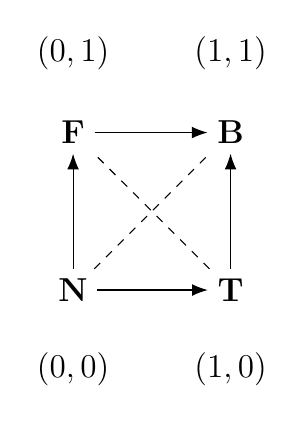
\begin{tikzpicture}[scale=2, every node/.style={font=\large}]
  \node (N) at (0,0) {$\Nval$};
  \node (T) at (1,0) {$\Tval$};
  \node (F) at (0,1) {$\Fval$};
  \node (B) at (1,1) {$\Bval$};
  \draw[-{Latex[length=2mm]}] (N) -- (T);
  \draw[-{Latex[length=2mm]}] (N) -- (F);
  \draw[-{Latex[length=2mm]}] (T) -- (B);
  \draw[-{Latex[length=2mm]}] (F) -- (B);
  \draw[dashed] (N) -- (B);
  \draw[dashed] (T) -- (F);
  \node[below=4mm of N] {$(0,0)$};
  \node[below=4mm of T] {$(1,0)$};
  \node[above=4mm of F] {$(0,1)$};
  \node[above=4mm of B] {$(1,1)$};
\end{tikzpicture}
\end{center}

Define the threshold-wall count
\[
  \dthr(a,b)
  =\mathbf{1}[a^+\neq b^+]
   +\mathbf{1}[a^-\neq b^-].
\]
Lean verifies the basic geometry:
\[
  0\le \dthr(a,b)\le 2,
\]
\[
  \dthr(a,b)=0\iff a=b,
\]
and
\[
  \dthr(a,b)=2
  \iff
  a^+\neq b^+\ \land\ a^-\neq b^-.
\]
Thus one-wall changes are exactly edge moves and two-wall changes are exactly diagonal moves. The two diagonal pairs are
\[
  \Nval\leftrightarrow\Bval,
  \qquad
  \Tval\leftrightarrow\Fval.
\]

\begin{proposition}[Robustness is zero displacement]
Every compositionally robust modal formula has threshold-wall count zero under its designated admissible conditionalization.
\statusverified
\end{proposition}

The reachability construction realizes every displacement class. Hence the dynamic picture combines two properties that might initially look opposed:
\[
  \text{global categorical reachability is complete,}
\]
while
\[
  \text{local categorical change is exactly coordinatewise threshold change.}
\]
This tension is the starting point for the geometric refinement in the next sections.

\section{From Threshold Straddling to Literal Affine Crossings}
\label{sec:affine}

The Boolean square records which threshold decisions differ, but it does not yet say what numerical event lies behind a changed bit. The next formal layer reconnects categorical displacement to rational support masses.

\subsection{Endpoint straddling}

For a rational threshold \(c\), define
\[
  \operatorname{Straddle}(c;x,y)
\]
to mean that exactly one endpoint lies on or above the threshold:
\[
  (c\le x\land\neg(c\le y))
  \ \lor\ 
  (c\le y\land\neg(c\le x)).
\]
For rational numbers this is the expected endpoint pattern
\[
  x<c\le y
  \quad\text{or}\quad
  y<c\le x.
\]

\begin{theorem}[Threshold decision versus endpoint straddling]
For rational \(c,x,y\),
\[
  [c\le x]\neq[c\le y]
  \iff
  \operatorname{Straddle}(c;x,y).
\]
\statusverified
\end{theorem}

At belief level, the total wall count decomposes into the one-dimensional wall counts of the positive and negative support coordinates. Lean therefore verifies the exact three-way correspondence:
\[
\begin{array}{ccl}
\dthr=0 &\iff& \text{neither support coordinate straddles},\\
\dthr=1 &\iff& \text{exactly one support coordinate straddles},\\
\dthr=2 &\iff& \text{both support coordinates straddle}.
\end{array}
\]
In particular, every genuine categorical belief change has a numerical endpoint witness on at least one signed support axis.

\subsection{Affine interpolation}

Endpoint straddling still describes only two snapshots. To expose an actual crossing event, the formalization introduces the directed rational affine path
\[
  \gamma_{x,y}(t)=x+t(y-x),
  \qquad t\in\mathbb{Q}.
\]
It satisfies
\[
  \gamma_{x,y}(0)=x,
  \qquad
  \gamma_{x,y}(1)=y.
\]

For the increasing orientation \(x<c\le y\), the explicit threshold parameter is
\[
  t_+=\frac{c-x}{y-x}.
\]
For the decreasing orientation \(y<c\le x\), the development uses the equivalent directed parameter
\[
  t_- =\frac{x-c}{x-y}.
\]
Lean Core rational arithmetic is sufficient to prove that the relevant parameter lies in the unit interval and hits the threshold exactly.

\begin{theorem}[Affine unit-interval threshold crossing]
If rational endpoints \(x,y\) straddle rational threshold \(c\), then
\[
  \exists t\in\mathbb{Q}:
  0\le t\le 1
  \quad\land\quad
  \gamma_{x,y}(t)=c.
\]
\statusverified
\end{theorem}

\begin{proof}[Proof sketch]
Straddling implies distinct endpoints. Solve \(x+t(y-x)=c\) for \(t=(c-x)/(y-x)\); the straddling inequalities give \(0\le t\le1\), accounting for the sign of the denominator. Substitution verifies the hit. A hit can be at an endpoint; the theorem does not require \(0<t<1\).
\end{proof}
No abstract topology is used, and there is no Mathlib dependency.

\begin{corollary}[Belief change has a literal affine wall hit]
If admissible conditionalization changes the complete FDE value of \(\Bel_i\varphi\), then at least one of the two chosen interpolations of its endpoint support masses
\[
  t\mapsto \Ppos_t(\varphi),
  \qquad
  t\mapsto \Pneg_t(\varphi)
\]
hits \(c_i\) at some rational \(t\in[0,1]\). Here \(\Ppos_t=(1-t)\Ppos_0+t\Ppos_1\), and likewise for negative support; this notation does not yet denote evaluation in an intermediate model.
\statusverified
\end{corollary}

For a two-wall transition, both signed support coordinates have crossing witnesses, though they need not cross at the same parameter. This asks an order question about the chosen interpolation: which wall is hit first?

\paragraph{Support-plane picture.}
The two masses define a point
\[
  (\Ppos,\Pneg)\in\mathbb{Q}^2.
\]
The threshold lines \(\Ppos=c\) and \(\Pneg=c\) partition the plane into the four FDE regions.

\begin{center}
\begin{tikzpicture}[scale=1.25]
  \draw[->] (0,0) -- (5,0) node[right] {$\Ppos$};
  \draw[->] (0,0) -- (0,5) node[above] {$\Pneg$};
  \draw[dashed] (2.4,0) -- (2.4,5) node[above] {$\Ppos=c$};
  \draw[dashed] (0,2.4) -- (5,2.4) node[right] {$\Pneg=c$};
  \node at (1.2,1.2) {$\Nval$};
  \node at (3.7,1.2) {$\Tval$};
  \node at (1.2,3.7) {$\Fval$};
  \node at (3.7,3.7) {$\Bval$};
  \fill (2.4,2.4) circle (1.5pt);
  \node[above right] at (2.4,2.4) {$(c,c)$};
\end{tikzpicture}
\end{center}

The threshold square is the four-region categorical observation of the signed support plane. These four regions must not be confused with the four evidence masses \((t,b,n,f)\) in a probability simplex. For integrity-certified models the relevant support points lie in the unit square; the algebraic lemmas themselves permit arbitrary rational coordinates.

\section{Unique Crossing Times and Temporal Order}
\label{sec:crossing-order}

A two-wall transition gives one affine threshold hit on the positive support coordinate and one on the negative coordinate. To turn these hits into a temporal classification, the crossing parameter must be intrinsic rather than an arbitrary existential witness.

\subsection{Uniqueness}

Suppose \(x\neq y\). The affine map
\[
  \gamma_{x,y}(t)=x+t(y-x)
\]
is injective in its parameter. Lean proves this directly over the rationals by cancelling the nonzero factor \(y-x\).

\begin{theorem}[Unique affine threshold time]
Let \(x\neq y\). If
\[
  \gamma_{x,y}(t)=c
  \qquad\text{and}\qquad
  \gamma_{x,y}(s)=c,
\]
then
\[
  t=s.
\]
Consequently every straddling affine segment has a unique threshold crossing parameter in \([0,1]\cap\mathbb{Q}\).
\statusverified
\end{theorem}

For a two-wall belief transition write
\[
  t_+=\text{the unique positive-support crossing time},
\]
\[
  t_-=\text{the unique negative-support crossing time}.
\]
Both lie in the rational unit interval.

\subsection{Crossing-order trichotomy}

The linear order on \(\mathbb{Q}\) now yields an exhaustive classification:
\[
  t_+<t_-,
  \qquad
  t_+=t_-,
  \qquad
  t_-<t_+.
\]

\begin{theorem}[Affine crossing-order trichotomy]
Every two-wall conditionalized belief transition admits intrinsic positive and negative crossing times satisfying exactly one of
\[
  t_+<t_-,\qquad
  t_+=t_-,\qquad
  t_-<t_+.
\]
\statusverified
\end{theorem}

The three cases have immediate event readings:
\[
\begin{array}{ccl}
 t_+<t_- &:& \text{positive threshold wall first},\\
 t_+=t_- &:& \text{simultaneous crossing},\\
 t_-<t_+ &:& \text{negative threshold wall first}.
\end{array}
\]

\subsection{The simultaneous case}

The equality case has a geometric characterization stronger than mere coincidence of two stored parameters.

\begin{theorem}[Simultaneity as the wall intersection]
For a two-coordinate affine crossing pair,
\[
  t_+=t_-
\]
if and only if there exists one rational parameter \(t\) such that
\[
  \Ppos_t=c
  \qquad\text{and}\qquad
  \Pneg_t=c.
\]
Equivalently, the support path passes through the wall-intersection point
\[
  (c,c).
\]
\statusverified
\end{theorem}

Thus simultaneous diagonal motion is geometrically exceptional. If \(t_+\neq t_-\), there is a nonempty rational interval between the two wall events. The next section proves that this interval carries a forced categorical phase.

\paragraph{Why order matters.}
The endpoint projection forgets which threshold coordinate changes first. Yet for a diagonal transition both bits must change. The temporal order of those changes therefore contains information absent from the pair \((\text{source},\text{target})\). Crossing-order geometry recovers exactly that lost information.

\section{Intermediate FDE Phases Between Sequential Crossings}
\label{sec:intermediate}

Suppose a two-wall transition is not simultaneous. The two unique crossing times then determine an open interval in which exactly one threshold coordinate has already switched to its target side.

The formal development chooses the rational midpoint
\[
  t_m=\frac{t_++t_-}{2}.
\]
If \(t_+<t_-\), Lean proves
\[
  t_+<t_m<t_-.
\]
If \(t_-<t_+\), the symmetric inequalities hold. These midpoint facts require only rational arithmetic.

\subsection{Threshold side before and after a crossing}

The affine support coordinate is strictly monotone whenever its endpoints are distinct. For an increasing straddling path, parameters before the unique crossing remain below threshold and parameters after it lie above threshold. For a decreasing path, the threshold sides reverse. The formal result can be stated without choosing an orientation:

\begin{proposition}[Source side before, target side after]
Let a rational affine support coordinate straddle \(c\) and hit \(c\) uniquely at time \(t_c\). Then
\[
  t<t_c
  \quad\Longrightarrow\quad
  \side_c(\gamma(t))=\side_c(x),
\]
and
\[
  t_c<t
  \quad\Longrightarrow\quad
  \side_c(\gamma(t))=\side_c(y).
\]
\statusverified
\end{proposition}

This is the key bridge from event order to a categorical intermediate state.

\subsection{Generic intermediate vertices}

Let
\[
  s=(s^+,s^-),
  \qquad
  t=(t^+,t^-)
\]
be opposite vertices of the threshold square. Define
\[
  I_+(s,t)=(t^+,s^-)
\]
for positive-first motion and
\[
  I_-(s,t)=(s^+,t^-)
\]
for negative-first motion.

\begin{theorem}[Positive-first midpoint phase]
If both support coordinates straddle and \(t_+<t_-\), then at the rational midpoint
\[
  \text{state}(t_m)=I_+(s,t).
\]
That is, the positive coordinate has already reached the target threshold side while the negative coordinate is still on the source threshold side.
\statusverified
\end{theorem}

\begin{theorem}[Negative-first midpoint phase]
If both support coordinates straddle and \(t_-<t_+\), then
\[
  \text{state}(t_m)=I_-(s,t).
\]
\statusverified
\end{theorem}

For opposite endpoints, both intermediate states are adjacent to source and target:
\[
  \dthr(s,I_\pm(s,t))=1,
  \qquad
  \dthr(I_\pm(s,t),t)=1.
\]
Hence every sequential diagonal displacement decomposes into two one-wall phases.

\subsection{Concrete diagonal table}

The complete verified table is:

\begin{center}
\begin{tabular}{ccc}
\toprule
Diagonal transition & positive wall first & negative wall first\\
\midrule
\(\Nval\to\Bval\) & \(\Tval\) & \(\Fval\)\\
\(\Bval\to\Nval\) & \(\Fval\) & \(\Tval\)\\
\(\Tval\to\Fval\) & \(\Nval\) & \(\Bval\)\\
\(\Fval\to\Tval\) & \(\Bval\) & \(\Nval\)\\
\bottomrule
\end{tabular}
\end{center}

Thus, for example,
\[
  \Nval\to\Bval
\]
can have either phase sequence
\[
  \Nval\to\Tval\to\Bval
\]
or
\[
  \Nval\to\Fval\to\Bval,
\]
and the choice is determined exactly by whether positive or negative support crosses the Lockean wall first.

% Reproducible study figure for the verified affine crossing-order results.
% Threshold c = 0.6. The three affine paths are chosen to illustrate
% positive-first, negative-first, and simultaneous N -> B transitions.
\begin{figure}[t]
\centering
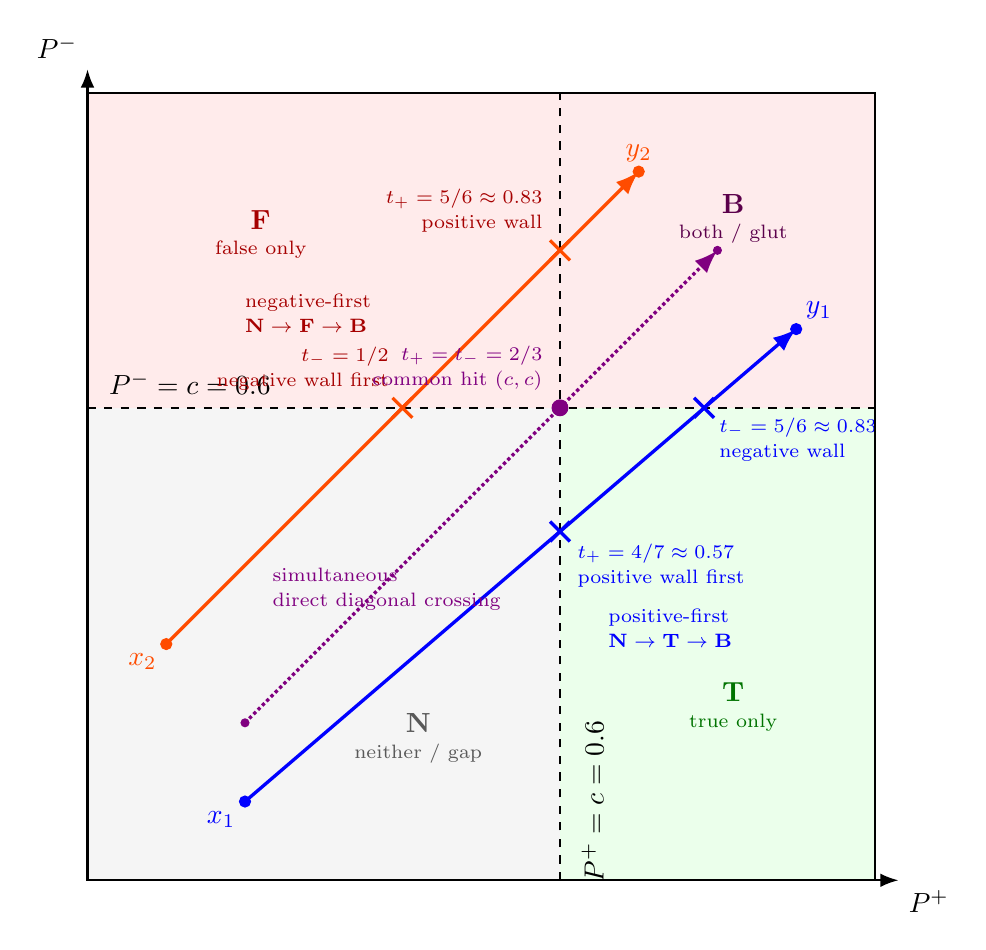
\begin{tikzpicture}[x=10cm,y=10cm,>=Latex]
  % Four threshold cells.
  \fill[black!4] (0,0) rectangle (0.6,0.6);
  \fill[green!8] (0.6,0) rectangle (1,0.6);
  \fill[red!8] (0,0.6) rectangle (0.6,1);
  \fill[blue!5!red!8] (0.6,0.6) rectangle (1,1);

  % Axes and threshold walls.
  \draw[->,thick] (0,0) -- (1.03,0) node[below right] {$P^+$};
  \draw[->,thick] (0,0) -- (0,1.03) node[above left] {$P^-$};
  \draw[dashed,thick] (0.6,0) -- (0.6,1);
  \draw[dashed,thick] (0,0.6) -- (1,0.6);
  \node[below,rotate=90] at (0.615,0.10) {$P^+=c=0.6$};
  \node[above] at (0.13,0.605) {$P^-=c=0.6$};

  % Cell labels.
  \node[align=center,text=black!65] at (0.42,0.18)
    {$\Nval$\\[-1mm]\scriptsize neither / gap};
  \node[align=center,text=green!45!black] at (0.82,0.22)
    {$\Tval$\\[-1mm]\scriptsize true only};
  \node[align=center,text=red!65!black] at (0.22,0.82)
    {$\Fval$\\[-1mm]\scriptsize false only};
  \node[align=center,text=blue!45!red!65!black] at (0.82,0.84)
    {$\Bval$\\[-1mm]\scriptsize both / glut};

  % Positive-first path: (0.2,0.1) -> (0.9,0.7).
  \draw[blue,very thick,->] (0.2,0.1) -- (0.9,0.7);
  \filldraw[blue] (0.2,0.1) circle (0.007);
  \filldraw[blue] (0.9,0.7) circle (0.007);
  \node[blue,below left] at (0.2,0.1) {$x_1$};
  \node[blue,above right] at (0.9,0.7) {$y_1$};
  % t_+ = 4/7, point (0.6, 31/70 ~= 0.443)
  \draw[blue,very thick] (0.6,0.443) node[draw,cross out,minimum size=6pt,inner sep=0pt] {};
  \node[blue,below right,align=left] at (0.61,0.44)
    {\scriptsize $t_+=4/7\approx0.57$\\[-1mm]\scriptsize positive wall first};
  % t_- = 5/6, point (47/60 ~= 0.783, 0.6)
  \draw[blue,very thick] (0.783,0.6) node[draw,cross out,minimum size=6pt,inner sep=0pt] {};
  \node[blue,below right,align=left] at (0.79,0.60)
    {\scriptsize $t_-=5/6\approx0.83$\\[-1mm]\scriptsize negative wall};

  % Negative-first path: (0.1,0.3) -> (0.7,0.9).
  \draw[red!70!yellow,very thick,->] (0.1,0.3) -- (0.7,0.9);
  \filldraw[red!70!yellow] (0.1,0.3) circle (0.007);
  \filldraw[red!70!yellow] (0.7,0.9) circle (0.007);
  \node[red!70!yellow,below left] at (0.1,0.3) {$x_2$};
  \node[red!70!yellow,above] at (0.7,0.9) {$y_2$};
  % t_- = 1/2 at (0.4,0.6)
  \draw[red!70!yellow,very thick] (0.4,0.6) node[draw,cross out,minimum size=6pt,inner sep=0pt] {};
  \node[red!65!black,above left,align=right] at (0.395,0.61)
    {\scriptsize $t_-=1/2$\\[-1mm]\scriptsize negative wall first};
  % t_+ = 5/6 at (0.6,0.8)
  \draw[red!70!yellow,very thick] (0.6,0.8) node[draw,cross out,minimum size=6pt,inner sep=0pt] {};
  \node[red!65!black,above left,align=right] at (0.59,0.81)
    {\scriptsize $t_+=5/6\approx0.83$\\[-1mm]\scriptsize positive wall};

  % Simultaneous path: (0.2,0.2) -> (0.8,0.8), common hit at t=2/3.
  \draw[blue!50!red,densely dotted,very thick,->] (0.2,0.2) -- (0.8,0.8);
  \filldraw[blue!50!red] (0.2,0.2) circle (0.005);
  \filldraw[blue!50!red] (0.8,0.8) circle (0.005);
  \filldraw[blue!50!red] (0.6,0.6) circle (0.010);
  \node[blue!50!red,above left,align=right] at (0.59,0.61)
    {\scriptsize $t_+=t_-=2/3$\\[-1mm]\scriptsize common hit $(c,c)$};

  % Path labels in free regions.
  \node[blue,align=left] at (0.74,0.32)
    {\scriptsize positive-first\\[-1mm]\scriptsize $\Nval\to\Tval\to\Bval$};
  \node[red!65!black,align=left] at (0.28,0.72)
    {\scriptsize negative-first\\[-1mm]\scriptsize $\Nval\to\Fval\to\Bval$};
  \node[blue!50!red,align=left] at (0.38,0.37)
    {\scriptsize simultaneous\\[-1mm]\scriptsize direct diagonal crossing};

  % Unit-square frame.
  \draw[thick] (0,0) rectangle (1,1);
\end{tikzpicture}
\caption{Affine phase geometry for three $\Nval\to\Bval$ support trajectories at threshold $c=0.6$.  Positive-first and negative-first paths necessarily occupy $\Tval$ and $\Fval$, respectively, between their unique wall-crossing times.  The simultaneous path is the exceptional case $t_+=t_-$ and passes through the wall intersection $(c,c)$.  The figure is a visualization of the Lean-verified crossing-order and intermediate-phase theorems; it does not by itself assert that every interpolated support point is already realized by a full admissible model.}
\label{fig:fde-phase-geometry}
\end{figure}


Figure~\ref{fig:fde-phase-geometry} makes the trichotomy explicit for three rational affine trajectories with the same threshold. The two sequential cases pass through different adjacent FDE cells, whereas the simultaneous path hits the unique wall intersection and therefore has no open interval carrying an intermediate adjacent phase.

\begin{theorem}[Two-wall intermediate-phase classification]
Every two-wall conditionalized belief transition admits an affine crossing pair such that either
\begin{enumerate}[label=(\roman*)]
  \item the two crossing times are equal and the support path hits \((c,c)\), or
  \item the positive crossing is earlier and the midpoint has the positive-first intermediate FDE state, or
  \item the negative crossing is earlier and the midpoint has the negative-first intermediate FDE state.
\end{enumerate}
\statusverified
\end{theorem}

\paragraph{Critical semantic boundary.}
The theorem classifies the explicit affine interpolation of the two support masses. It does not yet prove that the midpoint support pair is generated by a complete intermediate 4-PEL model satisfying all model and update constraints. Accordingly, the phrase ``intermediate epistemic phase'' refers here to the thresholded support state along the verified affine support trajectory, not yet to a model-valued dynamical path.

\section{From Probability Simplexes to Strong Model Paths}
\label{sec:model-paths}

The affine crossing results of the previous sections are formulated at the level of signed support masses. To interpret those trajectories as genuine probabilistic model trajectories, the probability layer must first satisfy more than the lightweight normalization contract built into the original \texttt{Model} structure. This section records the stronger layer and the verified lift from rational weight vectors to complete 4-PEL models.

\subsection{Finite probability integrity}

The compatibility predicate \texttt{FiniteProbabilityIntegrity} strengthens one local measure by requiring duplicate-free support, nonnegative event masses, extensionality with respect to event membership, monotonicity, disjoint finite additivity, empty-event mass zero, and total support mass one. The wrapper \texttt{StrongProbabilityModel} equips an ordinary 4-PEL model with this stronger certification.

The stronger contract is deliberately additive rather than a replacement of the legacy model interface. Earlier finite witnesses therefore remain available, while later geometric results can state explicitly when genuine finite-probability behavior is required.

\begin{proposition}[Weight-generated finite probability]
Let \(R\) be a duplicate-free finite support and let \(q:R\to\mathbb{Q}\) be nonnegative with total mass one. Define the mass of a finite event \(S\) by summing the weights of the points of \(R\) that belong to \(S\). Then the resulting local measure satisfies \texttt{FiniteProbabilityIntegrity}.
\statusverified
\end{proposition}

The implementation iterates over the fixed support rather than over the event list. Consequently event order and duplicate presentation do not alter the generated mass.

\subsection{Convexity of the finite probability simplex}

For two valid weight distributions \(q_0,q_1\) on the same support and rational \(t\in[0,1]\), define
\[
  q_t(x)=(1-t)q_0(x)+tq_1(x).
\]
Lean verifies that \(q_t\) is again a valid finite weight distribution. Hence the full rational line segment between two valid endpoints remains in the finite probability simplex.

More strongly, every fixed event mass is affine in the same parameter:
\[
  \mu_t(S)
  =(1-t)\mu_0(S)+t\mu_1(S).
\]

\begin{theorem}[Affine event mass on the probability simplex]
For every fixed event \(S\), the weight-generated mass along the convex distribution path satisfies
\[
  \mu_{q_t}(S)
  =(1-t)\mu_{q_0}(S)+t\mu_{q_1}(S).
\]
\statusverified
\end{theorem}

This identity is the formal bridge between the probability simplex and the affine scalar paths used in the threshold-crossing theorems.

\subsection{A model-valued rational path}

The probability path can be lifted to the complete model structure. Fix a world list \(W\), an accessibility field \(R\), an atomic valuation \(v\), and Lockean thresholds \(c\). Let \(q_0\) and \(q_1\) provide valid local weight distributions at every agent/world pair. For every rational \(t\in[0,1]\), define
\[
  M_t=(W,R,\mu_t,v,c),
\]
where each local measure is generated from the interpolated weights \(q_t\).

\begin{theorem}[Convex strong model path]
Every rational \(t\in[0,1]\) determines a \texttt{StrongProbabilityModel} \(M_t\). Along the entire path,
\[
  W_t=W,
  \qquad
  R_t=R,
  \qquad
  v_t=v,
  \qquad
  c_t=c,
\]
and every fixed local event has affine probability mass.
\statusverified
\end{theorem}

Thus the geometric probability path is realized by complete probabilistically certified 4-PEL models, rather than merely by pairs of numbers in a support plane.

\paragraph{Exact scope of the realization.}
Two distinctions remain essential. First, this theorem concerns weight-generated strong endpoint models on a common semantic skeleton. It does not retroactively prove that every legacy witness in the repository satisfies the stronger probability contract. Second, a convex model path is not the same thing as an update-generated path: the theorem does not claim that every intermediate \(M_t\) arises by conditionalizing the source model on some evidence event.

The first formula-level lift is also verified. If \(\varphi\) is
probability-free, its value depends only on accessibility and atomic valuation,
which remain fixed along the path. Hence its positive and negative support
events are fixed, and Lean proves
\[
  \Ppos_t(\varphi)=(1-t)\Ppos_0(\varphi)+t\Ppos_1(\varphi),
  \qquad
  \Pneg_t(\varphi)=(1-t)\Pneg_0(\varphi)+t\Pneg_1(\varphi).
\]

These two scalar identities are now packaged into the rational support
coordinate
\[
  z_\varphi(M,i,w)=\Ppos_M(\varphi)+i\Pneg_M(\varphi).
\]

\begin{theorem}[Affine complex support on strong model paths]
For every probability-free modal formula and every rational \(t\in[0,1]\),
the complete strong model path satisfies
\[
  z_\varphi(M_t,i,w)
  =(1-t)z_\varphi(M_0,i,w)+t z_\varphi(M_1,i,w).
\]
The equality is componentwise in \texttt{ComplexCoord Rat}.
\statusverified
\end{theorem}

Thus the complex support trajectory is itself a model-level affine object, not
merely an informal pairing of two separately affine quantities. The notation
\(i\) here remains coordinate notation; no probabilistic or object-language
complex multiplication is introduced.

The remaining formula-level boundary concerns formulas containing
probabilistic belief. Their own values, and therefore their support events, can
vary with \(t\). The next formal step is to lift the crossing-order and
intermediate-phase theorems through this coordinate directly to the strong
model path.

\section{Structural Interpretation: From Reachability to Phase Kinematics}
\label{sec:interpretation}

\statusinterpretive

The formal results support a layered interpretation of four-valued epistemic change. At the finest level considered here, a belief formula is represented by two rational support masses. Thresholding projects this point into one of four regions. The resulting FDE value forgets the precise probabilities and remembers only which side of the two Lockean walls each coordinate occupies.

This can be written as a coarse-graining map
\[
  q_c:\mathbb{Q}^2\longrightarrow\{\Tval,\Fval,\Bval,\Nval\},
\]
\[
  q_c(p^+,p^-)
  =([p^+\ge c],[p^-\ge c]).
\]
The two threshold lines partition the support plane into four cells. The Boolean threshold square is the adjacency graph of these cells. In this sense the four-valued state space is not an arbitrary collection of labels. It is the quotient of a signed evidence space by two threshold predicates.

\subsection{Global freedom, local constraint}

Two verified results together give the central dynamic contrast:
\[
  \text{every ordered categorical transition is realizable},
\]
while
\[
  \text{every categorical change is mediated by a threshold-side change}.
\]
Global reachability is therefore maximal, but local motion is not structureless. A transition leaves a trace in the signed support coordinates. Zero-wall movement is robust, one-wall movement crosses one categorical boundary, and two-wall movement crosses both.

The affine results sharpen this further. A diagonal transition does not merely differ in both bits. Along the chosen support interpolation it contains two unique wall events. Those events may coincide, or they may be temporally ordered. If they are ordered, a forced adjacent phase lies between them. The endpoint displacement therefore hides a short event history.

It is useful to call this structure \emph{epistemic phase kinematics}. The term is not an additional theorem. It names the combination of four verified layers:
\[
  \text{cell membership},
  \quad
  \text{wall count},
  \quad
  \text{crossing time},
  \quad
  \text{intermediate phase sequence}.
\]

\subsection{The exceptional role of simultaneity}

For a diagonal move, sequential crossings force an intermediate adjacent phase. Simultaneity is the unique way in which this ordered two-step decomposition disappears. Geometrically, simultaneity requires the affine support path to pass through the codimension-two intersection \((c,c)\). It is therefore a special alignment condition in the support plane rather than the generic consequence of changing both bits.

This distinction may become important in later model-level dynamics. If admissible model paths can realize the affine support interpolation, sequential diagonal changes would carry genuine intermediate epistemic states, while simultaneous changes would behave as boundary-coincident transitions.

\subsection{Connection to structural transport}

A broader working hypothesis in the 4-PEL project treats epistemic paradoxes as failures of structural transport. The present dynamic results fit that program in a precise but limited way. Thresholding is a projection from rich signed probabilistic information to a coarse four-valued state. Endpoint states alone do not preserve crossing order. Recovering the order requires returning to the richer support trajectory.

The paper does not claim that all epistemic paradoxes reduce to threshold crossing. Rather, this case study supplies one clean instance of a recurring pattern:
\[
  \text{rich structure}
  \longrightarrow
  \text{coarse projection}
  \longrightarrow
  \text{apparent categorical jump},
\]
where restoring the discarded structure reveals the mechanism hidden by the projection.

The formal contribution of the present paper ends before this philosophical generalization. A general structural-transport theorem connecting threshold dynamics to the project’s other paradox families remains open.

\section{Lean Mechanization and Verification Status}
\label{sec:mechanization}

The artifact uses Lean 4.31.0 without Mathlib. The current branch is
\texttt{research/modal-probabilistic-fine-graining}; the root module
\texttt{PEL4.lean} imports the relevant development. Appendix~\ref{app:formal}
provides the claim-to-declaration map, including the reliability refinement.
The explicit audit files are the machine-readable list of selected claims;
this selection is not a certification of every declaration in the repository.

\subsection{Verification contract}
A successful build establishes that declarations typecheck, not that all their
assumptions are proved. Version 0.4 therefore audits 52 manuscript declarations
in \texttt{PEL4/PaperAxiomAudit.lean} and 24 MPFG declarations in its separate
audit. The full build and both strict audits passed for source revision
\texttt{07fbc5193e0f7e43de565158c0eaf0cbb9c08dfb}; the review report records the
CI run and exact dependencies. Only \texttt{propext}, \texttt{Classical.choice},
and \texttt{Quot.sound}, or subsets thereof, occur in these selected chains.
\texttt{sorryAx}, project-specific axioms, and native-decision axioms are rejected.

The review found that some general headlines inherited native-evaluation
assumptions through elementary helpers. In eight source modules, the relevant
finite computations were changed from \texttt{native\_decide} to
\texttt{decide +kernel}, without changing statements or semantic definitions.
Legacy declarations outside the audited chains may still use native evaluation
or project axioms; no repository-wide axiom-freedom claim is made.

\subsection{Status discipline}
The manuscript follows the repository verification policy:
\begin{enumerate}[label=(\arabic*)]
\item \textbf{PROVED}: the stated theorem typechecks and its audited dependency
chain contains no project-specific unproved assumption. Explicit hypotheses
and model proof fields remain assumptions of the theorem's quantified statement.
\item \textbf{FINITE-WITNESS}: a finite construction or counterexample is
verified. Finite domain coverage is not a theorem about arbitrary model sizes.
\item \textbf{EXPERIMENTAL / INTERPRETIVE}: terminology, philosophical readings,
and prospective extensions without a corresponding established theorem.
\item \textbf{AXIOMATIC-PROTOTYPE}: a substantive property is postulated.
No manuscript headline is promoted from this category merely because it compiles.
\end{enumerate}
The proof sketches explain the main arguments for readers; Lean verifies their
formal counterparts. The geometry uses rational algebra, not topological
continuity. Numerical figure coordinates illustrate those statements and are
not additional model-realization certificates.

\paragraph{Reproducibility.}
From a clean clone, or after preserving local work:
\begin{verbatim}
git fetch origin
git switch research/modal-probabilistic-fine-graining
git pull --ff-only
lake build
python3 scripts/check_mpfg_axioms.py
python3 scripts/check_paper_axioms.py --report paper-axioms.json
python3 -m unittest discover -s scripts -p 'test_*.py'
cd paper
latexmk -pdf -interaction=nonstopmode -halt-on-error main.tex
\end{verbatim}
The mutable branch is for ongoing development; use a recorded commit for an
exact reproduction. Lean checking and manuscript rendering remain separate
checks. The committed PDF is the rendered working artifact, not evidence of
formal correctness by itself.

\section{Related Work, Limits, and Open Problems}
\label{sec:limits}

The semantic kernel belongs to the Belnap--Dunn/FDE tradition of tracking support for truth and falsity independently \cite{Belnap1977,Dunn1976}. Four-valued modal logics with bilateral relational semantics have been studied in several forms \cite{OdintsovWansing2010,RivieccioJungJansana2017}. The present project adds a finite probabilistic threshold layer and a primitive evidence-stable knowledge operator whose behavior is analyzed mechanically rather than assumed to coincide with a standard modal box.

The threshold connection between all-or-nothing belief and degrees of belief belongs to the broader Lockean tradition. Leitgeb's stability theory is a particularly important point of comparison because it places stability conditions at the interface between probability and categorical belief \cite{Leitgeb2014}. The 4-PEL notion of stability is different in type: it concerns invariance of the complete FDE value across an accessible profile and acts as a filter from threshold belief to knowledge. A careful conceptual comparison is therefore needed before stronger claims about similarity or difference are made.

The update perspective is adjacent to dynamic epistemic logic, where informational actions transform epistemic models and knowledge states \cite{vanDitmarschHoekKooi2007}. The conditionalization operator studied here is narrower: it preserves worlds, accessibility, valuation, and threshold and changes only local probabilities. Conversely, the four-valued signed-support geometry developed here is not part of the standard DEL vocabulary. The manuscript reports this construction without claiming that it is novel relative to all probabilistic or nonclassical dynamic epistemic systems.

\paragraph{Novelty boundary.}
No strong novelty claim is made in this version. The individual mathematical ingredients are elementary: Boolean pairs, threshold comparisons, affine interpolation, finite convex probability, linear order, and midpoint arguments. The research contribution currently established internally to the project is the machine-checked composition of these ingredients into one dependency chain connecting admissible probabilistic update to four-valued categorical reachability, robustness, crossing order, intermediate phase structure, and a model-valued rational probability path. A systematic literature audit is publication-critical.

\subsection{Verified model-path layer and remaining realization questions}

The earlier support-to-model existence problem now has a positive answer for a precise class. Given two weight-generated strong endpoint models on the same semantic skeleton, rational convex interpolation of their local weights produces a \texttt{StrongProbabilityModel} for every \(t\in[0,1]\cap\mathbb{Q}\). Worlds, accessibility, valuation, and threshold remain fixed, and the probability of every fixed event varies affinely.

Two stronger realization questions remain open.

\begin{question}[Formula-level support realization]
For which modal formulas \(\varphi\) are the positive and negative support events invariant along a convex strong model path, so that the verified affine fixed-event theorem applies directly to \(\Ppos_t(\varphi)\) and \(\Pneg_t(\varphi)\)?
\end{question}

Atomic propositions are the natural first case because their valuation is fixed by construction. A broader probability-free fragment is plausible but requires an explicit theorem connecting path-invariance of \texttt{evalModal} to fixed support-event membership.

\begin{question}[Update-generated path]
When can the intermediate models of a convex strong model path themselves be obtained by admissible conditionalization of the source model, possibly using a parameterized family of evidence events?
\end{question}

A model-valued path and an update-generated path are different notions. C17D verifies the former and deliberately does not infer the latter.

\subsection{Open problem 2: arbitrary continuous paths}

The affine crossing theorem is constructive and sufficient for the present phase result, but it is not a general topological theorem. A stronger layer would define a continuous support path
\[
  \gamma:[0,1]\to\mathbb{R}^2
\]
and prove that endpoint straddling forces intersection with the appropriate threshold wall. Standard intermediate-value reasoning would then recover a crossing theorem independent of linear interpolation.

For two-wall transitions, arbitrary paths introduce genuinely new geometry. A path may meet the two walls multiple times, touch a wall without changing side, or revisit a categorical cell. The current uniqueness and three-case temporal order are specific to nonconstant affine coordinates. A general theory would therefore need a richer notion of crossing event than the present unique hit parameter.

\subsection{Open problem 3: algebraic stability}

The knowledge filter is presently defined semantically by full-value homogeneity over an accessible range. An open problem is to characterize this stability intrinsically in bilattice or algebraic terms and to determine which logical operators preserve, reflect, or destroy it. Such a characterization could connect the dynamic phase table to existing algebraic semantics for four-valued modal systems.

\subsection{Open problem 4: higher-dimensional phase complexes}

A single belief formula contributes two threshold bits. For \(n\) tracked formulas, the naive categorical state space has \(2n\) threshold coordinates and therefore resembles a Boolean hypercube. This suggests a higher-dimensional generalization of wall count, crossing order, and phase sequence. Dependencies between formulas, however, can identify or forbid regions of that cube. Determining the realizable cell complex is a natural extension of the present two-dimensional result.

\subsection{Open problem 5: structural transport and paradox families}

The project contains independent formal diagnoses of Lottery, Preface, Sorites, Knower, Surprise Examination, Moore/Fitch, and dynamic threshold phenomena. The working phrase ``paradoxes as failures of structural transport'' is currently interpretive. A genuine general theorem would require an abstract account of transformations, observations, preserved predicates, and counterexamples that subsumes several of these families without erasing their differences.

\section{A conservative modal-probabilistic refinement gate}
\label{sec:mpfg}

This extension is a semantic refinement of evidence, not a replacement of the
four-valued algebra. Its formal declarations are in
\texttt{PEL4/ModalProbability/Refinement.lean} and
\texttt{PEL4/ModalProbability/StatusTransport.lean}.
The gate's validation status is recorded in
\texttt{docs/MODAL\_PROBABILISTIC\_FINE\_GRAINING.md}.

\begin{definition}[Reliability-tagged evidence profile]
A fine profile is a nonnegative rational vector
\(q=(t,b,n,f,t_r,f_r)\) of total mass one. Its coarse projection is
\[
  \pi(q)=(t+t_r,b,n,f+f_r).
\]
The reliability tags are supplied semantic data, not proofs of empirical
truth. The untagged lift of \((t,b,n,f)\) is \((t,b,n,f,0,0)\).
\end{definition}

Consequently \(\pi\) has a right inverse. Signed support is preserved:
\(P^+(q)=t+t_r+b\) and \(P^-(q)=f+f_r+b\).
For \(0\le a\le1\), both normalized rational simplexes are closed under mixing,
and the formal projection identity is
\[
 \pi((1-a)q+ar)=(1-a)\pi(q)+a\pi(r).
\]
Thus raw threshold belief commutes with forgetting reliability. This does not
assert that thresholding is affine; the raw belief compatibility follows from
the chosen definitions. Moreover, no function of the coarse profile recovers
reliable mass \(t_r+f_r\) in general: pure untagged truth and pure reliable truth
have the same projection, but reliable masses zero and one.

\begin{definition}[Status stability and local fibre rigidity]
For any relation \(R\), observation \(v\), and projection \(\pi\), put
\begin{align*}
 \mathrm{Stable}(v,w)
   &\iff \forall u\,(Rwu\Rightarrow v(u)=v(w)),\\
 \mathrm{Rigid}(v,\pi,w)
   &\iff \forall u\,(Rwu\Rightarrow
       (\pi(v(u))=\pi(v(w))\Rightarrow v(u)=v(w))).
\end{align*}
\end{definition}

The exact transport boundary is
\[
 \mathrm{Stable}(v,w)\iff
 \mathrm{Stable}(\pi\circ v,w)\land\mathrm{Rigid}(v,\pi,w).
\]
This is a local decomposition, not a claim that fibre rigidity is automatic.
Two universally accessible worlds carrying untagged and reliable truth witness
coarse stability with fine instability, even on a reflexive, transitive,
Euclidean frame. A second witness distinguishes mass stability from categorical
stability: \((0,1,0,0)\) and \((0,3/4,1/4,0)\) both yield \(\Bval\) at threshold
\(3/5\), although their glut masses differ.

The auxiliary essence predicate means conditionally retaining the current
specified status across accessible worlds; it may hold vacuously. Its accidental
counterpart requires an actual different accessible status. These are classical
meta-level predicates, not additional FDE connectives. Their relationship to
the existing executable stability test and \(\Know\) is stated separately:
applying the unchanged knowledge interpretation to raw fine belief or to its
coarse projection yields the same value. No identification of \(\Know\) with
ordinary S5 necessity is made.

Finally, the existing finite-step-chain theorem transports threshold status
when each edge preserves it. Cell refinement is distinct from population
Finite Fine-Grainedness, and connectivity alone does not imply status
preservation. Normalized reliability-sensitive updates, probability-one versus
necessity under full-support assumptions, and any representation of
proof-theoretic fractional values remain subsequent research targets.

\section{Matroidal evidence closure}
\label{sec:matroid-evidence}

The four-valued kernel records whether positive and negative evidence are
present, but it does not by itself distinguish evidential novelty from coarse
repetition. This section adds a structural layer for that distinction. The
claim is deliberately restricted: arbitrary bodies of epistemic evidence are
\emph{not} assumed to form matroids. Instead, the bilateral 4-PEL signature
canonically induces a two-channel closure structure. The formal declarations
are in \texttt{PEL4/MatroidEvidence.lean}, with a separate declaration-level
trust inventory in \texttt{PEL4/MatroidEvidenceAxiomAudit.lean}.

\begin{definition}[Two-channel evidence closure]
Let \(E\) be a type of evidence atoms and let
\(\chi:E\to\{+,-\}\) assign each atom its coarse 4-PEL polarity. For
\(A\subseteq E\), define
\[
  \operatorname{cl}_{\chi}(A)
  = \{e\in E : \exists a\in A\;\chi(a)=\chi(e)\}.
\]
Thus, after coarse projection, one item of positive evidence generates the
whole positive parallel class, and likewise for negative evidence. No claim is
made that the underlying fine-grained sources are interchangeable.
\end{definition}

\begin{theorem}[4-PEL channel closure]
The operator \(\operatorname{cl}_{\chi}\) is extensive, monotone, idempotent,
and satisfies the closure exchange law
\[
 x\in \operatorname{cl}_{\chi}(A\cup\{y\}),\quad
 x\notin \operatorname{cl}_{\chi}(A)
 \quad\Longrightarrow\quad
 y\in \operatorname{cl}_{\chi}(A\cup\{x\}).
\]
Hence the coarse positive/negative partition carries a matroid closure
presentation. In particular,
\[
 y\in \operatorname{cl}_{\chi}(\{x\})
 \quad\Longleftrightarrow\quad
 \chi(x)=\chi(y).
\]
\textup{\textsc{Status: Lean-proved; separate declaration-level audit in
\texttt{PEL4/MatroidEvidenceAxiomAudit.lean}.}}
\end{theorem}
\begin{proof}[Proof sketch]
Extensivity and monotonicity follow immediately from retaining a witness of the
same polarity. Idempotence collapses a two-step same-polarity witness to a
one-step witness. For exchange, if \(x\) enters the closure only after inserting
\(y\), then the witnessing atom cannot already belong to \(A\); consequently
\(x\) and \(y\) have the same polarity, so inserting \(x\) places \(y\) in the
closure. This is the two-class partition instance of the standard closure
view of matroids \cite{Whitney1935,Oxley2011}.
\end{proof}

For a body of evidence \(A\), write
\(\operatorname{Supp}_{+}(A)\) and \(\operatorname{Supp}_{-}(A)\) for the
existence of positive and negative atoms respectively. These two predicates
recover exactly the bilateral Boolean observations used by the FDE kernel.

\begin{proposition}[Coarse-state conservativity]
For each polarity \(\sigma\in\{+,-\}\),
\[
  \operatorname{Supp}_{\sigma}(\operatorname{cl}_{\chi}(A))
  \quad\Longleftrightarrow\quad
  \operatorname{Supp}_{\sigma}(A).
\]
Consequently, if \(A\) realizes an FDE value by matching its positive and
negative bits to these two support predicates, then
\(\operatorname{cl}_{\chi}(A)\) realizes exactly the same value, and conversely.
Matroidal closure removes coarse redundancy without changing the four-valued
observation.
\textup{\textsc{Status: Lean-proved; separate declaration-level audit in
\texttt{PEL4/MatroidEvidenceAxiomAudit.lean}.}}
\end{proposition}

\begin{proposition}[Channel-rank profile]
Define the coarse channel rank of \(v\) as the number of present bilateral
support bits. Then
\[
  r(\Nval)=0,\qquad
  r(\Tval)=r(\Fval)=1,\qquad
  r(\Bval)=2.
\]
\textup{\textsc{Status: Lean-proved by reduction.}}
\end{proposition}

The rank profile changes the interpretation of contradiction in a useful way.
At this coarse structural level, \(\Bval\) is not deficient in evidence: it has
maximal channel rank because both independent directions are represented.
Paraconsistency is therefore compatible with high evidential breadth. Rank
alone is not a truth value, however. Since \(\Tval\) and \(\Fval\) both have
rank one, polarity orientation remains essential. The rank statistic measures
how many coarse evidence directions are represented, not which direction they
support and not how reliable or numerous their sources are.

\paragraph{Scope boundary.}
Same-polarity atoms are parallel only after projection to the two bits observed
by the FDE kernel. Two independent laboratories, two proofs, or two sensors may
remain genuinely distinct at a finer epistemic level even when both contribute
positive support. The present theorem therefore establishes a canonical
\emph{coarse} matroid induced by 4-PEL; it does not establish the general thesis
that evidence, justification, or information always has matroid structure.
Reliability tags, source identity, probabilistic weight, and inferential origin
are intentionally outside this first gate.

\subsection{Gate 2: the topological exchange boundary}
\label{sec:matroid-topological-boundary}

The repository also contains a topological evidence semantics in which an
algebraic interior operator induces a closure \(\operatorname{cl}\). That closure
is extensive, monotone, idempotent, and preserves binary unions. The last fact
makes the interaction with matroid exchange unusually rigid. Let
\[
  x\preceq_{\operatorname{cl}} y
  \quad\Longleftrightarrow\quad
  x\in\operatorname{cl}(\{y\}).
\]
For a genuine point-set topology this is the specialization preorder (up to the
usual orientation convention). Symmetry of this preorder is the standard
\(R_0\) separation condition \cite{Willard1970}.

\begin{theorem}[Topological exchange characterization]
For the topological closure generated by an \texttt{InteriorSemantics}, the
following are equivalent:
\begin{enumerate}[label=(\roman*)]
  \item the closure satisfies the Mac Lane--Steinitz exchange condition;
  \item singleton specialization is symmetric:
  \[
    x\in\operatorname{cl}(\{y\})
    \quad\Longrightarrow\quad
    y\in\operatorname{cl}(\{x\}).
  \]
\end{enumerate}
Thus, for ordinary topological spaces, the repository-level matroid exchange
boundary is exactly the \(R_0\) boundary.
\textup{\textsc{Status: Lean-proved in
\texttt{PEL4/MatroidTopologicalBridge.lean}; declaration-level audit included.}}
\end{theorem}
\begin{proof}[Proof sketch]
Since topological closure preserves binary unions,
\[
  \operatorname{cl}(A\cup\{y\})
  =\operatorname{cl}(A)\cup\operatorname{cl}(\{y\}).
\]
If \(x\) enters the closure only after adjoining \(y\), then
\(x\in\operatorname{cl}(\{y\})\); singleton symmetry gives
\(y\in\operatorname{cl}(\{x\})\), hence
\(y\in\operatorname{cl}(A\cup\{x\})\). Conversely, exchange over the empty
base sends \(x\in\operatorname{cl}(\{y\})\) to
\(y\in\operatorname{cl}(\{x\})\), because the topological closure of the empty
set is empty.
\end{proof}

This result distinguishes two forms of ``being generated by nearby evidence.''
Topological closure may encode directional approximation: one point can lie in
the closure of another without reciprocal dependence. Matroid exchange forbids
that asymmetry at the singleton level. In a genuine \(T_0\) topology, adding the
exchange condition therefore pushes the singleton specialization relation to
equality, i.e. to the \(T_1\) boundary.

\begin{proposition}[Sierpiński obstruction]
The two-point Sierpiński topology already used as a finite witness in the 4-PEL
topological semantics does not satisfy matroid exchange. At its distinguished
points,
\[
  \mathsf{focus}\in\operatorname{cl}(\{\mathsf{neighbour}\}),
  \qquad
  \mathsf{neighbour}\notin\operatorname{cl}(\{\mathsf{focus}\}).
\]
Hence singleton specialization is asymmetric, so the topological closure fails
exchange.
\textup{\textsc{Status: Lean-proved in
\texttt{PEL4/MatroidTopologicalSierpinski.lean}.}}
\end{proposition}

The obstruction is internal to the existing 4-PEL topological research line;
it is not an unrelated topology introduced solely to refute exchange. The same
Sierpiński witness previously exposed directional boundary behaviour for
\(\Box\) and \(\Diamond\), and Gate 2 now identifies that directionality as the
precise reason the closure is not matroidal.

\begin{proposition}[Channel topology realization]
The coarse Gate-1 positive/negative channel matroid is itself topological.
Define
\[
  \operatorname{Int}_{\chi}(A)
  =\{e : \forall a\,(\chi(a)=\chi(e)\Rightarrow a\in A)\}.
\]
This is the partition topology generated by the polarity classes, and its dual
closure satisfies
\[
  \operatorname{cl}_{\operatorname{Int}_{\chi}}(A)
  =\operatorname{cl}_{\chi}(A).
\]
Its singleton specialization relation is symmetric and therefore satisfies
exchange.
\textup{\textsc{Status: Lean-proved in
\texttt{PEL4/MatroidTopologicalBridge.lean}.}}
\end{proposition}

Gate 2 therefore locates the original channel matroid inside the intersection
of the two structural programs: it is simultaneously a partition-topological
closure and a matroidal closure. The Sierpiński semantics lies outside that
intersection. This gives the 4-PEL evidence layer a first nontrivial structural
boundary rather than merely two parallel mathematical descriptions.

\paragraph{Formal scope.}
The repository's \texttt{MatroidClosure} is intentionally a lightweight
closure-axiom presentation and currently does not add a finite-character axiom.
The characterization above is therefore a theorem about exactly that formal
notion. On the finite carriers used by the explicit 4-PEL witnesses, finite
character is automatic; infinite-carrier finitarity remains a separate
extension.

\paragraph{Next structural questions.}
The next natural gate is combinatorial rather than topological: formalize
matroid circuits as minimal dependent evidence sets and determine what a
minimal evidential redundancy means in 4-PEL. After that, deletion and
contraction can be tested as formal models of removing an evidence source and
quotienting by accepted background evidence. A further question is whether the
six-cell reliability refinement preserves the \(R_0\)-like exchange boundary
under coarse projection.

\section{Circuits as minimal evidential redundancy}
\label{sec:matroid-circuits}

Gate~2 identified the exact topological boundary at which the coarse 4-PEL
closure also satisfies matroid exchange. Gate~3 turns from closure geometry to
combinatorial dependence. In matroid theory a circuit is a minimal dependent
set \cite{Whitney1935,Oxley2011}. For the two-channel 4-PEL projection this
notion admits a particularly sharp interpretation: a circuit is a smallest body
of evidence containing a coarse redundancy that disappears as soon as either of
its members is removed.

\begin{definition}[Channel dependence]
Let \(\chi:E\to\{+,-\}\) be the coarse evidence polarity. A body of evidence
\(A\subseteq E\) is \emph{channel-dependent} when
\[
  \exists x,y\in A\quad x\neq y
  \quad\text{and}\quad
  \chi(x)=\chi(y).
\]
It is channel-independent when no such pair exists. A \emph{channel circuit}
is a channel-dependent set with no proper channel-dependent subset.
\end{definition}

The definition is equivalent to the expected closure formulation.

\begin{proposition}[Closure witness for dependence]
For every \(A\subseteq E\),
\[
  A\text{ is channel-dependent}
  \quad\Longleftrightarrow\quad
  \exists x\in A:\
  x\in\operatorname{cl}_{\chi}(A\setminus\{x\}).
\]
Thus coarse dependence means that at least one retained atom is already generated
by the remainder of the evidence body.
\textup{\textsc{Status: Lean-proved in
\texttt{PEL4/MatroidEvidenceCircuits.lean}.}}
\end{proposition}

\begin{theorem}[Complete circuit classification]
A body \(C\subseteq E\) is a channel circuit if and only if there exist distinct
\(x,y\in E\) such that
\[
  \chi(x)=\chi(y)
  \qquad\text{and}\qquad
  C=\{x,y\}.
\]
Equivalently, the circuits of the coarse 4-PEL partition matroid are exactly the
two-element same-polarity pairs.
\textup{\textsc{Status: Lean-proved in
\texttt{PEL4/MatroidEvidenceCircuits.lean}.}}
\end{theorem}
\begin{proof}[Proof sketch]
Every distinct same-polarity pair is dependent. Any dependent subset of that
pair must contain two distinct elements, so it must contain both members and
therefore equals the pair. Conversely, if \(C\) is minimally dependent, choose
two distinct same-polarity witnesses \(x,y\in C\). The pair \(\{x,y\}\) is
already dependent, hence minimality forces every member of \(C\) to lie in that
pair. Since both witnesses lie in \(C\), equality follows.
\end{proof}

This theorem turns the informal phrase ``redundant evidence'' into an exact
structural claim. At the coarse bilateral projection, a circuit does not mean
that one item of evidence is false, weak, or dispensable in every epistemic
sense. It means only that two distinct atoms occupy the same one-bit direction
seen by the FDE kernel.

\begin{proposition}[Circuit closure redundancy]
If \(x\neq y\) and \(\chi(x)=\chi(y)\), then for every \(e\in E\),
\[
  e\in\operatorname{cl}_{\chi}(\{x,y\})
  \quad\Longleftrightarrow\quad
  e\in\operatorname{cl}_{\chi}(\{x\}).
\]
By symmetry the same holds with \(\{y\}\). Hence removing either member of a
circuit leaves the coarse generated channel unchanged.
\textup{\textsc{Status: Lean-proved.}}
\end{proposition}

The circuit-elimination behaviour is correspondingly transparent. Suppose
\(\{x,y\}\) and \(\{x,z\}\) are distinct circuits sharing \(x\). Then all three
atoms have the same polarity; if \(y\neq z\), the pair \(\{y,z\}\) is itself a
circuit contained in the union after removing the common element. This is the
two-channel instance of the standard circuit-elimination pattern
\cite{Oxley2011}.

\begin{proposition}[Two-channel circuit elimination]
Let \(x,y,z\) be pairwise distinct with
\(\chi(x)=\chi(y)=\chi(z)\). Then
\[
  \{x,y\},\{x,z\}\text{ circuits}
  \quad\Longrightarrow\quad
  \{y,z\}\text{ is a circuit}.
\]
\textup{\textsc{Status: Lean-proved.}}
\end{proposition}

\subsection{Contraction as accepted background evidence}

Deletion and contraction are the canonical minor operations of matroid theory.
The current repository interface, however, presents only a closure operator and
has no explicit ground-set field. A full minor API would therefore be premature:
removing an atom from the carrier cannot yet be represented without changing the
ambient type or extending \texttt{MatroidClosure}. Gate~3 instead records the
part of contraction semantics that is expressible without pretending that this
missing structure already exists.

Fix an evidence atom \(c\) and treat it as accepted background evidence. Define
\[
  \operatorname{cl}_{\chi}^{/c}(A)
  :=\operatorname{cl}_{\chi}(A\cup\{c\}).
\]
This is a contraction-style background closure rather than a packaged matroid
minor.

\begin{proposition}[Parallel evidence becomes loop-like under background]
For any atom \(e\),
\[
  \chi(c)=\chi(e)
  \quad\Longrightarrow\quad
  e\in\operatorname{cl}_{\chi}^{/c}(\varnothing),
\]
whereas
\[
  \chi(c)\neq\chi(e)
  \quad\Longrightarrow\quad
  e\notin\operatorname{cl}_{\chi}^{/c}(\varnothing).
\]
Thus accepting one positive atom as background makes every positive parallel
atom generated without further evidence, while negative atoms remain a separate
information direction; and conversely for negative background evidence.
\textup{\textsc{Status: Lean-proved.}}
\end{proposition}

This is the strongest epistemic reading justified by the present formalism. In
a genuine contraction of a partition matroid, the parallel partners of the
contracted element become loops. Here the formal result captures exactly the
corresponding closure fact: once one channel representative is fixed in the
background, additional same-channel atoms contribute no new coarse rank.

\paragraph{Gate-3 boundary.}
The classification is exact only after the positive/negative projection. At a
finer level, two positive reports may differ in reliability, causal origin,
probability mass, inferential route, or independence of source. Such information
can split a coarse two-element circuit into an independent fine-grained set.
Consequently, ``minimal evidential redundancy'' is always indexed to a chosen
projection.

\paragraph{Next structural question.}
Gate~4 should promote the lightweight closure presentation to an explicit
finite-ground-set matroid layer, or bridge the project to a standard matroid API.
Only then can deletion and contraction be stated as actual minors rather than
background-closure probes. That gate would allow a precise comparison between
source removal, background acceptance, rank loss, loop creation, and preservation
of the four-valued state.

\section{Conclusion}
\label{sec:conclusion}

The case study establishes three bounded results. First, the stipulated evidence-stable knowledge operator factors through accessible-profile homogeneity; probability-only conditionalization realizes all sixteen \(\Know(\Bel p)\) endpoint values across a six-world witness family. This is not a claim that one fixed model realizes every update, nor an empirical theory of knowledge.

Second, signed thresholding reduces quantitative support to two Boolean decisions. On a chosen rational affine segment, straddling gives unique wall-hit parameters and their order determines a sequential midpoint phase. An actual discrete update does not supply this interpolated history. At simultaneous hits the inclusive threshold yields \(\Bval\), which may occur only at the boundary parameter.

Separately, normalized rational world weights construct probability-integrity-certified model paths with affine fixed-event masses. Connecting these paths to the supports of arbitrary probability-sensitive formulas, or generating them by admissible updates, remains unproved. The weakest model interface is not silently promoted to a finite probability space.

Third, six-cell reliability tagging preserves coarse support and convex mixing but loses recoverable reliability under projection. Fine current-world stability holds exactly when coarse stability and local fibre rigidity both hold. The S5-frame witnesses show that frame geometry alone cannot restore discarded information. The tags are supplied semantic data, not a derivation of reliability or a six-valued logical calculus.

The contribution is a reproducible mechanized analysis of preservation and information loss. The declaration-level audits, explicit finite witnesses, and proof sketches identify what is established and under which contract. Before journal submission, the most valuable next steps are a strong certificate for the reachability family, a formula-level model-path bridge, and a theorem-by-theorem comparison with the probability and evidence-logics literature. No claim of completeness, topological generality, or priority is inferred from a successful build.


\appendix
\section{Formal Correspondence}
\label{app:formal}

This appendix maps the principal mathematical claims in the manuscript to the Lean modules and theorem names that support them. The list is selective rather than exhaustive. All names below are in namespace \texttt{PEL4}; the audit files enumerate exact fully qualified targets. A theorem's hypotheses remain part of its claim.

\begingroup
\small
\begin{longtable}{@{}p{0.28\textwidth}p{0.31\textwidth}p{0.31\textwidth}@{}}
\toprule
Paper claim & Lean theorem / definition & Module\\
\midrule
Four FDE values as bilateral Boolean pairs & \texttt{FDEValue}, \texttt{FDEValue.T/F/B/N} & \texttt{PEL4/FDE.lean}\\
\addlinespace
Signed threshold belief & \texttt{belief} & \texttt{PEL4/Belief.lean}\\
\addlinespace
Primitive modal evaluator with \(\Bel,\Know,\Diamond\) & \texttt{ModalFormula}, \texttt{evalModal} & \texttt{PEL4/ModalLanguage.lean}\\
\addlinespace
Knowledge equals stability-filtered belief & \texttt{modal\_knowledge\_as\_stability\_filtered\_belief} & \texttt{PEL4/ModalKnowledgeBeliefFactorization.lean}\\
\addlinespace
Safe probability-only update & \texttt{ConditionalizationAdmissible}, \texttt{conditionalize} & \texttt{PEL4/Dynamics.lean}\\
\addlinespace
Probability-free invariance & \texttt{evalModal\_conditionalize\_of\_probabilityFree} & \texttt{PEL4/ModalDynamicsStability.lean}\\
\addlinespace
Four dynamic stability phases & \texttt{modal\_knowledge\_phase\_stable\_stable}, \texttt{modal\_knowledge\_phase\_stable\_unstable}, \texttt{modal\_knowledge\_phase\_unstable\_stable}, \texttt{modal\_knowledge\_phase\_unstable\_unstable} & \texttt{PEL4/ModalDynamicsPhaseClassification.lean}\\
\addlinespace
Both stability-change directions are realizable & \texttt{conditionalization\_realizes\_both\_stability\_phase\_directions} & \texttt{PEL4/ModalDynamicsPhaseClassification.lean}\\
\addlinespace
All sixteen \(\Know(\Bel p)\) endpoint transitions & \texttt{conditionalization\_realizes\_every\_knowledge\_value\_transition} & \texttt{PEL4/ModalDynamicsReachability.lean}\\
\addlinespace
Creation of a knowledge glut & \texttt{conditionalization\_can\_create\_knowledge\_glut} & \texttt{PEL4/ModalDynamicsReachability.lean}\\
\addlinespace
Glut-to-gap and gap-to-truth transitions & \texttt{conditionalization\_can\_turn\_knowledge\_glut\_into\_gap}, \texttt{conditionalization\_can\_turn\_knowledge\_gap\_into\_truth} & \texttt{PEL4/ModalDynamicsReachability.lean}\\
\addlinespace
Exact belief robustness boundary & \texttt{modal\_belief\_value\_eq\_iff\_threshold\_bits\_eq} & \texttt{PEL4/ModalDynamicsRobustness.lean}\\
\addlinespace
Compositional robust formulas are invariant & \texttt{evalModal\_conditionalize\_of\_robust} & \texttt{PEL4/ModalDynamicsRobustness.lean}\\
\addlinespace
Robustness strictly extends the probability-free fragment & \texttt{diagonal\_reachability\_belief\_is\_robust}, \texttt{diagonal\_reachability\_belief\_not\_probabilityFree} & \texttt{PEL4/ModalDynamicsRobustness.lean}\\
\addlinespace
Threshold wall count & \texttt{thresholdWallCount} & \texttt{PEL4/ModalDynamicsGeometry.lean}\\
\addlinespace
Zero wall iff equal FDE state & \texttt{thresholdWallCount\_eq\_zero\_iff} & \texttt{PEL4/ModalDynamicsGeometry.lean}\\
\addlinespace
Two walls iff both coordinates flip & \texttt{thresholdWallCount\_eq\_two\_iff} & \texttt{PEL4/ModalDynamicsGeometry.lean}\\
\addlinespace
Wall flip iff endpoint straddling & \texttt{threshold\_decision\_ne\_iff\_straddles} & \texttt{PEL4/ModalDynamicsThresholdCrossing.lean}\\
\addlinespace
Two walls iff both supports straddle & \texttt{conditionalization\_belief\_two\_walls\_iff\_both\_supports\_straddle} & \texttt{PEL4/ModalDynamicsThresholdCrossing.lean}\\
\addlinespace
Affine path & \texttt{affineRatPath} & \texttt{PEL4/ModalDynamicsAffineCrossing.lean}\\
\addlinespace
Straddling gives unit-interval threshold hit & \texttt{thresholdStraddles\_has\_affine\_unit\_crossing} & \texttt{PEL4/ModalDynamicsAffineCrossing.lean}\\
\addlinespace
Every belief change has an affine wall hit & \texttt{conditionalization\_belief\_change\_has\_affine\_threshold\_crossing} & \texttt{PEL4/ModalDynamicsAffineCrossing.lean}\\
\addlinespace
Two-wall transition has two affine hits & \texttt{conditionalization\_belief\_two\_walls\_has\_two\_affine\_crossings} & \texttt{PEL4/ModalDynamicsAffineCrossing.lean}\\
\addlinespace
Unique affine threshold time & \texttt{affineRatPath\_threshold\_hit\_unique} & \texttt{PEL4/ModalDynamicsCrossingOrder.lean}\\
\addlinespace
Crossing-order trichotomy & \texttt{affineCrossingPair\_order\_trichotomy} & \texttt{PEL4/ModalDynamicsCrossingOrder.lean}\\
\addlinespace
Simultaneous iff common \((c,c)\) hit & \texttt{affineCrossingPair\_simultaneous\_iff\_common\_hit} & \texttt{PEL4/ModalDynamicsCrossingOrder.lean}\\
\addlinespace
Conditionalized two-wall order classification & \texttt{conditionalization\_belief\_two\_walls\_crossing\_order} & \texttt{PEL4/ModalDynamicsCrossingOrder.lean}\\
\addlinespace
Midpoint lies between sequential crossings & \texttt{affineCrossingMidpoint\_between\_positive\_first}, \texttt{affineCrossingMidpoint\_between\_negative\_first} & \texttt{PEL4/ModalDynamicsIntermediatePhase.lean}\\
\addlinespace
Source side before and target side after crossing & \texttt{affine\_threshold\_side\_before\_crossing\_eq\_source}, \texttt{affine\_threshold\_side\_after\_crossing\_eq\_target} & \texttt{PEL4/ModalDynamicsIntermediatePhase.lean}\\
\addlinespace
Positive-first midpoint state & \texttt{affineCrossingPair\_positive\_first\_midpoint\_state} & \texttt{PEL4/ModalDynamicsIntermediatePhase.lean}\\
\addlinespace
Negative-first midpoint state & \texttt{affineCrossingPair\_negative\_first\_midpoint\_state} & \texttt{PEL4/ModalDynamicsIntermediatePhase.lean}\\
\addlinespace
Intermediate is adjacent to both diagonal endpoints & \texttt{positiveFirstIntermediate\_adjacent\_to\_diagonal\_endpoints}, \texttt{negativeFirstIntermediate\_adjacent\_to\_diagonal\_endpoints} & \texttt{PEL4/ModalDynamicsIntermediatePhase.lean}\\
\addlinespace
Concrete eight-case diagonal table & \texttt{affine\_diagonal\_intermediate\_vertex\_table} & \texttt{PEL4/ModalDynamicsIntermediatePhase.lean}\\
\addlinespace
Full simultaneous/sequential intermediate-phase theorem & \texttt{conditionalization\_belief\_two\_walls\_intermediate\_phase} & \texttt{PEL4/ModalDynamicsIntermediatePhase.lean}\\
\addlinespace
Strong finite-probability contract & \texttt{FiniteProbabilityIntegrity}, \texttt{StrongProbabilityModel} & \texttt{PEL4/FiniteProbabilityIntegrity.lean}\\
\addlinespace
Weight-generated measure satisfies integrity & \texttt{weightGeneratedMeasure\_integrity} & \texttt{PEL4/WeightGeneratedProbability.lean}\\
\addlinespace
Convex interpolation preserves distributions & \texttt{convexWeightDistribution} & \texttt{PEL4/ConvexProbabilitySimplex.lean}\\
\addlinespace
Every fixed event mass is affine & \texttt{weightedEventMass\_convex} & \texttt{PEL4/ConvexProbabilitySimplex.lean}\\
\addlinespace
Complete strong rational model path & \texttt{convexStrongModelAt} & \texttt{PEL4/ConvexModelPath.lean}\\
\addlinespace
Worlds, accessibility, valuation, and threshold fixed & \texttt{convexStrongModelAt\_worlds}, \texttt{convexStrongModelAt\_accessibility}, \texttt{convexStrongModelAt\_valuation}, \texttt{convexStrongModelAt\_threshold} & \texttt{PEL4/ConvexModelPath.lean}\\
\addlinespace
Fixed-event mass affine along full model path & \texttt{convexStrongModelAt\_eventMass} & \texttt{PEL4/ConvexModelPath.lean}\\
\addlinespace
Nonempty accessibility and fixed-input K invariance & \texttt{PaperReview.accessibility\_nonempty}, \texttt{PaperReview.knowledge\_ignores\_probability\_for\_fixed\_values} & \texttt{PEL4/PaperReviewBoundaries.lean}\\
\addlinespace
Inclusive common hit is B; simultaneous T/F witness & \texttt{PaperReview.threshold\_intersection\_is\_B}, \texttt{PaperReview.simultaneous\_T\_F\_has\_B\_hit} & \texttt{PEL4/PaperReviewBoundaries.lean}\\
\addlinespace
Six-cell section and nonrecoverable reliability & \texttt{ModalProbability.SixCellProbability.coarse\_untagged}, \texttt{ModalProbability.SixCellProbability.no\_reliability\_reconstruction} & \texttt{PEL4/ModalProbability/Refinement.lean}\\
\addlinespace
Affine coarse projection & \texttt{ModalProbability.coarse\_mix} & \texttt{PEL4/ModalProbability/Refinement.lean}\\
\addlinespace
Local fine/coarse stability boundary & \texttt{ModalProbability.stable\_iff\_coarse\_and\_fibre\_rigid} & \texttt{PEL4/ModalProbability/StatusTransport.lean}\\
\addlinespace
S5-frame reliability and changing glut-mass witnesses & \texttt{ModalProbability.probability\_profile\_projection\_hides\_instability}, \texttt{ModalProbability.stable\_B\_does\_not\_mean\_constant\_mass} & \texttt{PEL4/ModalProbability/StatusTransport.lean}\\
\bottomrule
\end{longtable}
\endgroup

\paragraph{Verification note.}
The full Lean 4.31 CI build and strict audits described in Section~\ref{sec:mechanization} passed. The audited manuscript and MPFG declarations have only standard Lean axiom dependencies. Their statements, not informal paraphrases, determine the precise scope of verification. The formula-level lift from fixed events to arbitrary probability-sensitive support events remains separate and is not inferred from the model-path theorem.


\bibliographystyle{plain}
\bibliography{references}
\end{document}
